\documentclass[letterpaper,12pt,aspectratio=169,show notes,dvipsnames]{beamer}

% \setbeameroption{show notes on second screen=right}

\usepackage{amsmath}
\usepackage{amssymb}
\usepackage{amsthm}
\usepackage{attrib}
\usepackage{charter}
\usepackage{fontspec}
\usepackage{graphicx}
\usepackage{listings}
\usepackage{microtype}
\usepackage{multicol}
\usepackage{multirow}
\usepackage{natbib}
\usepackage{nicefrac}
\usepackage{proof}
\usepackage{tikz}
\usetikzlibrary{calc,shapes.callouts}
\usepackage{upquote}
\usepackage{xspace}

\setmainfont[Mapping=tex-text]{Noto Sans}
\newfontfamily\NotoSans[Mapping=tex-text]{Noto Sans}
\newfontfamily\NotoSerif[Mapping=tex-text]{Noto Serif}
\setmonofont{JuliaMono}

\mode<presentation>
{
  \useinnertheme{rectangles}
  \useoutertheme{default}
  \usecolortheme{whale}
  % \setbeamerfont{block title}{size=\large}
  \setbeamertemplate{itemize item}{\color{lime}$\blacktriangleright$}
  \setbeamertemplate{itemize subitem}{\color{olive}\scriptsize{$\blacktriangleright$}}
  % \setbeamercolor{titlelike}{parent=structure,bg=white!85!MSUgreen}
  % \setbeamercovered{transparent}
}

\addtobeamertemplate{navigation symbols}{}{%
  \usebeamerfont{footline}%
  \usebeamercolor[fg]{footline}%
  \hspace{1em}%
  {\scriptsize\insertframenumber/\inserttotalframenumber}
}  

\makeatletter
\setbeamertemplate{title page}{%
  \vbox{}
  \vfill
  \begingroup
  \centering
  \begin{beamercolorbox}[sep=8pt,center]{title}
    \usebeamerfont{title}\inserttitle\par%
    \ifx\insertsubtitle\@empty%
    \else%
      \vskip0.25em%
      {\usebeamerfont{subtitle}\usebeamercolor[fg]{subtitle}\insertsubtitle\par}%
    \fi%
  \end{beamercolorbox}%
  \vskip5em\par
  \begin{beamercolorbox}[sep=8pt,center]{author}
    \usebeamerfont{author}\insertauthor
  \end{beamercolorbox}
  % \begin{beamercolorbox}[sep=8pt,center]{institute}
  %   \usebeamerfont{institute}\insertinstitute
  % \end{beamercolorbox}
  % \begin{beamercolorbox}[sep=8pt,center]{date}
  %   \usebeamerfont{date}\insertdate
  % \end{beamercolorbox}\vskip0.5em
  \endgroup
  \vfill
}
\makeatother

\setbeamertemplate{section page}{
  \centering
  \begin{beamercolorbox}[sep=12pt,center]{section title}
    \usebeamerfont{section title}\insertsection\par
  \end{beamercolorbox}
}

\pgfkeys{/tikz/fulloverlay/.code={\pgfkeysalso{overlay, remember picture, shift=(current page.south west), x=(current page.south east), y=(current page.north west)}}}
\tikzset{
  invisible/.style={opacity=0,text opacity=0},
  visible on/.style={alt={#1{}{invisible}}},
  alt/.code args={<#1>#2#3}{%
    \alt<#1>{\pgfkeysalso{#2}}{\pgfkeysalso{#3}} % \pgfkeysalso doesn't change the path
  },
}

\colorlet{metaprogram}{violet}
\colorlet{linearity}{blue}
\colorlet{privacy}{orange}
\lstdefinelanguage{Elevator}%
{%
  morekeywords=%
  {%
    box, %
    lift, unlift,liftp,unliftp,%
    return,llet,let,in,%
    returnp,%
    Nat,suc,%
    NatArray,%
    fun,%
    if,then,else,%
    match,with,private%
  },%
  morecomment=[l]{\%},%
  moredelim=**[is][\color{metaprogram}]{m<<}{>>m},%
  moredelim=**[is][\color{linearity}]{l<<}{>>l},%
  moredelim=**[is][\color{privacy}]{p<<}{>>p},%
  moredelim=**[is][\color{violet}]{v<<}{>>v},%
  moredelim=**[is][\color{NavyBlue}]{nb<<}{>>nb},%
  moredelim=**[is][\color{WildStrawberry}]{ws<<}{>>ws},%
  sensitive,
}
\lstset{%
  basicstyle=\ttfamily\scriptsize,%
  keywordstyle=\bfseries,%
  literate=%
  {->}{{\(\rightarrow\)}}2 %
  {=>}{{\(\Rightarrow\)}}2 %
  {-o}{{\(\multimap\)}}2 %
  {^|}{{\(\uparrow\)}}2 %
  {v|}{{\(\downarrow\)}}2 %
  {b[]b}{{\(\Box\)}}2 % box
  {\\alpha}{{\(\alpha\)}}1 %
  {\\beta}{{\(\beta\)}}1 %
  {\\tau}{{\(\tau\)}}1 %
  {\\sigma}{{\(\sigma\)}}1 %
  {\\rho}{{\(\rho\)}}1 %
  ,%
  keepspaces=true,%
  numbers=left,%
  mathescape=true,%
  xleftmargin=0.05in,%
  resetmargins=true,%
  belowskip=0.05in,%
  aboveskip=0.05in,%
}
\lstloadlanguages{Elevator}
\lstset{language=Elevator}

\newcommand{\ctxEmpty}{{\cdot}}
\newcommand{\ctxCons}[2]{{#1 , #2}}
\newcommand{\ctxDrop}[2]{{#1 |_{#2}}}
% \newcommand{\ctxCut}[3]{{#1 \nmid^{#2} #3}}
\newcommand{\ctxCut}[3]{{#3 \ll^{#2}  #1}}
\newcommand{\ctxCutOp}[2]{(#1)\mid^{#2}}
\newcommand{\ctxWeaken}[1]{{\mathtt{weak}\ #1}}
% \newcommand{\ctxMerge}[3]{{#1 \boxplus #2 \Rightarrow #3}}
\newcommand{\ctxMerge}[3]{{#3 \Rightarrow #1 \boxplus #2 }}
\newcommand{\ctxUse}[3]{#1 \backslash #2 \Rightarrow #3}
% \newcommand{\ctxMode}[1]{{\underline{\mathsf{mode}}(#1)}}
% \newcommand{\ctxGe}[2]{{#1_{\ge{}#2}}}
% \newcommand{\ctxConv}[3]{{#1 \rightsquigarrow_{#2} {#3}}}

% \newcommand{\subst}[5]{{[#1 / #2]^{#3}_{#4} #5}}
\newcommand{\tmSub}[4]{[ #1 /^{#2} #3 ] #4}

\newcommand{\tyBox}[1]{{\Box #1}}
\newcommand{\tyBang}[1]{{! #1}}
\newcommand{\tyUp}[3]{{\uparrow^{#1}_{#2} #3}}
\newcommand{\tyDown}[3]{{\downarrow^{#1}_{#2} #3}}
\newcommand{\tyUnit}{{\mathtt{1}}}
\newcommand{\tyNat}{{\mathtt{Nat}}}
\newcommand{\tyLarr}[2]{{#1 \multimap #2}}
\newcommand{\tyArr}[2]{{#1 \to #2}}

\newcommand{\tmBangName}{!}
\newcommand{\tmBang}[1]{{\tmBangName #1}}
\newcommand{\tmLetbangName}{{\mathsf{let}\ !}}
\newcommand{\tmLetbang}[3]{{\tmLetbangName #1\ \mathsf{be}\ #2\ \mathsf{in}\ #3}}
\newcommand{\tmBoxName}{{\mathsf{box}}}
\newcommand{\tmBox}[1]{{\tmBoxName\ (#1)}}
\newcommand{\tmLetboxName}{{\mathsf{let}\ \mathsf{box}}}
\newcommand{\tmLetbox}[3]{{\tmLetboxName\ (#1) = #2\ \mathsf{in}\ #3}}
\newcommand{\tmLiftName}{{\mathsf{lift}}}
\newcommand{\tmLift}[3]{{\tmLiftName^{#1}_{#2}\ (#3)}}
\newcommand{\tmUnliftName}{{\mathsf{unlift}}}
\newcommand{\tmUnlift}[3]{{\tmUnliftName^{#1}_{#2}\ (#3)}}
\newcommand{\tmReturnName}{{\mathsf{return}}}
\newcommand{\tmReturn}[3]{{\tmReturnName^{#1}_{#2}\ (#3)}}
\newcommand{\tmLetreturnName}{{\mathsf{let}\ \mathsf{return}}}
\newcommand{\tmLetreturn}[5]{{\tmLetreturnName^{#1}_{#2}\ (#3) = #4\ \mathsf{in}\ #5}}
\newcommand{\tmUnit}{{\mathsf{unit}}}
\newcommand{\tmLam}[4]{{\lambda (#1 {:}^{#2} #3) . #4}}
\newcommand{\tmApp}[2]{{#1\ #2}}

\newcommand{\synDef}{{:=}}
\newcommand{\synOr}{{\ \ |\ \ }}
\newcommand{\synOrHead}{{|}}

\newcommand{\elevator}{\textsc{Elevator}\xspace}
\newcommand{\adjointcalctwo}{{\lambda^{\downarrow\uparrow2}}}
\newcommand{\modalcalc}{{\lambda^{\Box}}}

\newcommand{\modeSpec}{\mathcal{M}}
\newcommand{\modeOrdLt}[1][\modeSpec]{<^{#1}}
\newcommand{\modeOrdLe}[1][\modeSpec]{\le^{#1}}
\newcommand{\modeOrdGt}[1][\modeSpec]{>^{#1}}
\newcommand{\modeOrdGe}[1][\modeSpec]{\ge^{#1}}
\newcommand{\modeMapSt}[1][\modeSpec]{{\mathtt{st}_{#1}}}
\newcommand{\modeMapOp}[1][\modeSpec]{{\mathtt{op}_{#1}}}

\newcommand{\wknorm}[1]{\mathsf{WeakNorm}~(#1)}
\newcommand{\wkneut}[1]{\mathsf{WeakNeut}~(#1)}
\newcommand{\canon}[2]{\mathsf{Canon}^{#1}~(#2)}
\newcommand{\wf}[1]{\mathsf{wf}~(#1)}
\newcommand{\judg}[1]{\vdash^{#1}}
\newcommand{\algojudg}[1]{\,\,!\!\judg{#1}}
\newcommand{\equivMod}[6]{#1 \judg{#2} #4 \approx^{#3} #5 : #6}
\newcommand{\notEquivMod}[6]{#1 \judg{#2} #4 \not\approx^{#3} #5 : #6}

\AtBeginDocument{%
  \title{Adjoint Logic: Multiple Modalities into a Computational Framework}
  \date{}
  \author[J. Jang]{Junyoung Jang\\[0.2em]\scriptsize{junyoung.jang@mail.mcgill.ca}\\[0.2em]\scriptsize{McGill University}\\[1em]\scriptsize{Joint work with Brigitte Pientka}}
}

% =============================================================
% =============================================================

\bibliographystyle{plainnat}

\begin{document}
\begin{frame}
  \titlepage
\end{frame}

\begin{frame}{Adjoint Logic as a Uniform Framework}
  \color{black}
  \begin{tikzpicture}[fulloverlay]
    \node[visible on=<1->] at (0.3,0.45) {\(\mathtt{next}\) Modality};
    \node[visible on=<2->,alt=<3->{gray}{},text centered,text width=10em] at (0.3,0.37) {\footnotesize Binding-time Analysis\\[-0.2em]Model Checking};
    \node[visible on=<3->] at (0.5,0.65) {\(\Box\) Modality};
    \node[visible on=<4->,alt=<5->{gray}{}] at (0.5,0.6) {\footnotesize Staged programming};
    \node[visible on=<5->] at (0.7,0.45) {\(\bigcirc\) Modality};
    \node[visible on=<6->,alt=<7->{gray}{},text centered,text width=10em] at (0.7,0.37) {\footnotesize Information Flow\\[-0.2em]Reactive Programming};
    \draw[visible on=<8->,WildStrawberry] (0.5,0.45) ellipse (0.35 and 0.3);
    \node[visible on=<8->,WildStrawberry] at (0.5,0.77) {\large Adjoint Logic};

    \node[visible on=<9->,WildStrawberry,fill=white,draw] at (0.5,0.17) {\footnotesize while keeping static/dynamic semantics!};
  \end{tikzpicture}
\end{frame}

\begin{frame}{Adjoint Logic}
  \color{black}
  Uniform logic with two adjoint functors \(\tyUp{}{}{}\) (upshift)/\(\tyDown{}{}{}\) (downshift)\\connecting different sublogics:
  \pause
  \begin{itemize}[<+->]
  \item To connect linear and intuitionistic logic \citep{Benton:CSL94}
  \item To connect multiple logics in more general ways\citep{Reed09,Licata:LFCS16}
  \end{itemize}
  \pause
  \color{red} However,
  \begin{itemize}[<+->]
  \item \color{red} No decidable type checking
  \item \color{red} No syntactic operational/reduction semantics
  \item \color{red} No computational interpretation for \(\tyUp{}{}{}\)/\(\tyDown{}{}{}\)
  \end{itemize}
\end{frame}

\begin{frame}{\elevator \---- Adjoint Calculus in Action}
  \color{black}
  \textbf{Practical and uniform} foundation for programming inspired by adjoint logic
  \pause
  \begin{itemize}[<+->]
  \item Decidable type checking
  \item Operational semantics
  \item Computational interpretation for \(\tyUp{}{}{}\)/\(\tyDown{}{}{}\)
  \item Safety properties
  \item Embedding linear/affine types and \(\Box\)/\(\bigcirc\) types\\
    \pause
    while preserving static and dynamic semantics
  \end{itemize}
  \pause
\end{frame}

\begin{frame}{Overview of \elevator}
  \color{black}
  \begin{center}
    \scriptsize
    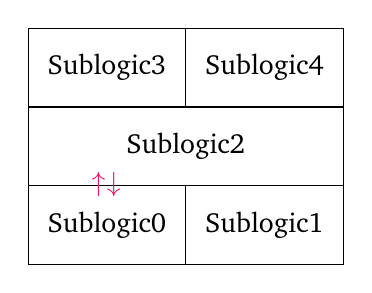
\begin{tikzpicture}
      \draw
      (0,2) rectangle (2,3)
      (2,2) rectangle (4,3)
      (0,1) rectangle (4,2)
      (0,0) rectangle (2,1)
      (2,0) rectangle (4,1);
      \node[alt=<3>{WildStrawberry}{}] (l0) at (1,0.5) {Sublogic0};
      \node (l1) at (3,0.5) {Sublogic1};
      \node[alt=<3>{WildStrawberry}{}] (l2) at (2,1.5) {Sublogic2};
      \node (l3) at (1,2.5) {Sublogic3};
      \node (l4) at (3,2.5) {Sublogic4};

      \node[visible on=<3>,WildStrawberry] at (1,1) {\(\tyUp{}{}{}\tyDown{}{}{}\)};
    \end{tikzpicture}
  \end{center}
  \scriptsize
  \begin{tikzpicture}[fulloverlay]
    \node[visible on=<2>,WildStrawberry,text centered,text width=18em] (desc0) at (0.8,0.75) {There are multiple sublogics\\each of which resides in one "mode"};
    \draw[visible on=<2>,->,WildStrawberry] (desc0.west) parabola (0.45,0.64);
    \draw[visible on=<2>,->,WildStrawberry] (desc0.west) parabola (0.57,0.64);

    \node[visible on=<3>,WildStrawberry,text centered,text width=22em] (desc1) at (0.2,0.29) {Adjoint modalities \(\tyUp{}{}{}\) and \(\tyDown{}{}{}\) allow\\ interaction between sublogics};
    \draw[visible on=<3>,->,WildStrawberry] (desc1.north) parabola[bend at end] (0.42,0.437);
  \end{tikzpicture}
\end{frame}

\begin{frame}{Mode Specification}
  \color{black}
  Modes are members of a {\color{violet}preorder}\\A mode controls allowed {\color{orange}structural rules} and {\color{blue}types} in a sublogic.\\[1em]

  \pause
  For example,
  \begin{center}
    \scriptsize
    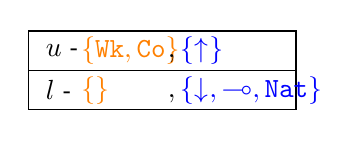
\begin{tikzpicture}[every node/.style=right]
      \draw
      (0,0.5) rectangle (3.4,1)
      (0,0) rectangle (3.4,0.5);
      \node (u) at (0.1,0.75) {\(u\) -};
      \node (um) at (0.55,0.75) {\(\color{orange}\{\mathtt{Wk}, \mathtt{Co}\}\)};
      \node (uo) at (1.65,0.75) {\(, \color{blue}\{\tyUp{}{}{}\}\)};
      \node (l) at (0.1,0.25) {\(l\) -};
      \node (lm) at (0.55,0.25) {\(\color{orange}\{\}\)};
      \node (lo) at (1.65,0.25) {\(, \color{blue}\{\tyDown{}{}{}, \tyLarr{}{}, \tyNat\}\)};
    \end{tikzpicture}
    \qquad
    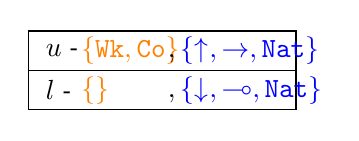
\begin{tikzpicture}[every node/.style=right]
      \draw
      (0,0.5) rectangle (3.4,1)
      (0,0) rectangle (3.4,0.5);
      \node (u) at (0.1,0.75) {\(u\) -};
      \node (um) at (0.55,0.75) {\(\color{orange}\{\mathtt{Wk}, \mathtt{Co}\}\)};
      \node (uo) at (1.65,0.75) {\(, \color{blue}\{\tyUp{}{}{}, \tyArr{}{}, \tyNat\}\)};
      \node (l) at (0.1,0.25) {\(l\) -};
      \node (lm) at (0.55,0.25) {\(\color{orange}\{\}\)};
      \node (lo) at (1.65,0.25) {\(, \color{blue}\{\tyDown{}{}{}, \tyLarr{}{}, \tyNat\}\)};
    \end{tikzpicture}
  \end{center}
  (where \({u \color{violet}\ge l}\))
  \scriptsize
  \begin{tikzpicture}[fulloverlay]
    \node[visible on=<3>,WildStrawberry] (dill) at (0.35,0.2) {\footnotesize Dual intuitionistic linear logic (DILL) \citep{Barber96}};
    \draw[visible on=<3>,->,WildStrawberry] (dill.north) -- (0.36,0.33);

    \node[visible on=<4>,WildStrawberry] (lnl) at (0.65,0.2) {\footnotesize Linear/non-linear logic (LNL) \citep{Benton:CSL94}};
    \draw[visible on=<4>,->,WildStrawberry] (lnl.north) -- (0.63,0.33);

    \node[visible on=<5>,violet] (hi) at (0.8,0.5) {Higher, More global, More long-lasting};
    \node[visible on=<5>,violet] (lo) at (0.8,0.28) {Lower, More local, More temporary};
    \draw[visible on=<5>,<-,violet] (hi.south) -- (lo.north);

    \node[visible on=<6-7>,right,orange] (wk) at (0.7,0.53) {Weakening};
    \draw[visible on=<6-7>,->,orange] (wk.west) parabola (0.59,0.435);

    \node[visible on=<8>,right,orange] (co) at (0.7,0.5) {Contraction};
    \draw[visible on=<8>,->,orange] (co.west) parabola (0.62,0.435);
  \end{tikzpicture}
\end{frame}

\begin{frame}{Mode Dependency Principle}
  \color{black}
  \begin{center}
	The behaviour of a sublogic of {\color{violet}a higher mode}\\cannot depend on\\the behaviour of a sublogic of {\color{violet}a lower mode}.
  \end{center}
\end{frame}

\begin{frame}{Adjoint Modalities \textemdash Computational Interpretation}
  \color{black}
  Adjoint modalities \(\tyUp{}{}{}\) and \(\tyDown{}{}{}\) connect two comparable modes:
  \pause
  \begin{itemize}[<+->]
  \item \(\tyUp{h}{l}{S}\) \textemdash{} \parbox{25em}{A thunk at a mode \(h\) of a closed deferred expression of type \(S\) at a lower mode \(l\)}\\[1em]
  \item \(\tyDown{h}{l}{S}\) \textemdash{} A pointer at a mode \(l\) to a stored value of type \(S\) at a higher mode \(h\)
  \end{itemize}
\end{frame}

\begin{frame}{Computational Interpretation of \(\tyUp{h}{l}{S}\)}
  \color{black}
  \pause
  \begin{itemize}
  \item<2-> \(\uncover<3->{\tmLift{h}{l}{L} : }\tyUp{h}{l}{S}\) \textemdash{} \parbox{22em}{A thunk at a mode \(h\) of a closed deferred expression \uncover<3->{\(L\)} of type \(S\) at a lower mode \(l\)}\\[1em]
  \item<4-> \(\tmUnlift{h}{l}{L} : S\) \textemdash{} compose/execute the expression in the thunk \(L : \tyUp{h}{l}{S}\)
  \end{itemize}
\end{frame}

\begin{frame}{Computational Interpretation of \(\tyDown{h}{l}{S}\)}
  \color{black}
  \pause
  \begin{itemize}
  \item<2-> \(\uncover<3->{\tmReturn{h}{l}{L} : }\tyDown{h}{l}{S}\) \textemdash{} \parbox{18em}{A pointer at a mode \(l\) to a stored value \uncover<3->{of \(L\)} of type \(S\) at a higher mode \(h\)}\\[1em]
  \item<4-> \(\tmLetreturn{h}{l}{x}{L}{M}\) \textemdash{} \parbox{19em}{load the value of type \(S\) referred by the pointer \(L : \tyDown{h}{l}{S}\) into \(x\) and continue with \(M\)}
  \end{itemize}
\end{frame}

\begin{frame}[fragile]{\(\lambda^{\Box}\) \textemdash A foundation for staged programming}
  \color{black}
  \begin{tikzpicture}[fulloverlay]
    \node[right] at (0.05,0.75) {\(\lambda^{\Box}\) \citep{Davies:ACM01}};
    \node[right] at (0.08,0.68) {\(\color{lime}\blacktriangleright\)\ \ \(\Box A\) describes a code fragment of type A};
    \node[visible on=<2>,right] at (0.33,0.5) {
      \begin{tikzpicture}[every node/.style=right,xscale=0.1,yscale=0.2,every node/.style={scale=1}]
        \draw
        (0,0.5) rectangle (3.4,1)
        (0,0) rectangle (3.4,0.5);
        \node (c) at (0.1,0.75) {\(c\) -};
        \node (cm) at (0.55,0.75) {\(\color{orange}\{\mathtt{Wk}, \mathtt{Co}\}\)};
        \node (co) at (1.65,0.75) {\(, \color{blue}\{\tyUp{}{}{}\}\)};
        \node (p) at (0.1,0.25) {\(p\) -};
        \node (pm) at (0.55,0.25) {\(\color{orange}\{\mathtt{Wk}, \mathtt{Co}\}\)};
        \node (po) at (1.65,0.25) {\(, \color{blue}\{\tyDown{}{}{}, \tyArr{}{}, \tyNat\}\)};
      \end{tikzpicture}
    };
  \end{tikzpicture}
\end{frame}

\begin{frame}[fragile]{Staging the Power Function}
  \color{black}
  \begin{tikzpicture}[fulloverlay]
    \node[visible on=<1->,right] at (0.05,0.75) {
      \begin{tikzpicture}[every node/.style=right,xscale=0.05,yscale=0.1,every node/.style={scale=0.5}]
        \draw
        (0,0.5) rectangle (3.4,1)
        (0,0) rectangle (3.4,0.5);
        \node (c) at (0.1,0.75) {\(c\) -};
        \node (cm) at (0.55,0.75) {\(\color{orange}\{\mathtt{Wk}, \mathtt{Co}\}\)};
        \node (co) at (1.65,0.75) {\(, \color{blue}\{\tyUp{}{}{}\}\)};
        \node (p) at (0.1,0.25) {\(p\) -};
        \node (pm) at (0.55,0.25) {\(\color{orange}\{\mathtt{Wk}, \mathtt{Co}\}\)};
        \node (po) at (1.65,0.25) {\(, \color{blue}\{\tyDown{}{}{}, \tyArr{}{}, \tyNat\}\)};
      \end{tikzpicture}
    };
    \node[visible on=<1>,right] at (0.1,0.5) {
\begin{lstlisting}
pow :$^p$ Nat -> nb<<v|$\color{NavyBlue}^c_p$^|$\color{NavyBlue}^c_p$>>nb(Nat -> Nat)
pow 0       =
  nb<<return$\color{NavyBlue}^c_p$>>nb (nb<<lift$\color{NavyBlue}^c_p$>>nb (fun x -> 1))
pow (suc n) =
  nb<<let return$\color{NavyBlue}^c_p$>>nb P = pow n nb<<in>>nb
  nb<<return$\color{NavyBlue}^c_p$>>nb (nb<<lift$\color{NavyBlue}^c_p$>>nb (fun x -> x * ((nb<<unlift$\color{NavyBlue}^c_p$>>nb P) x))
\end{lstlisting}
    };

    \node[visible on=<2>,right] at (0.1,0.5) {
\begin{lstlisting}
pow :$^p$ Nat -> ws<<v|$\color{WildStrawberry}^c_p$^|$\color{WildStrawberry}^c_p$>>ws(Nat -> Nat)
pow 0       =
  nb<<return$\color{NavyBlue}^c_p$>>nb (nb<<lift$\color{NavyBlue}^c_p$>>nb (fun x -> 1))
pow (suc n) =
  nb<<let return$\color{NavyBlue}^c_p$>>nb P = pow n nb<<in>>nb
  nb<<return$\color{NavyBlue}^c_p$>>nb (nb<<lift$\color{NavyBlue}^c_p$>>nb (fun x -> x * ((nb<<unlift$\color{NavyBlue}^c_p$>>nb P) x))
\end{lstlisting}
    };
    \node[visible on=<2>,right,WildStrawberry] (descBox) at (0.5,0.7) {\footnotesize Encoding of \(\Box\)};
    \draw[visible on=<2>,->,WildStrawberry] (descBox.west) parabola (0.3,0.62);

    \node[visible on=<3>,right] at (0.1,0.5) {
\begin{lstlisting}
pow :$^p$ Nat -> nb<<v|$\color{NavyBlue}^c_p$^|$\color{NavyBlue}^c_p$>>nb(Nat -> Nat)
pow 0       =
  nb<<return$\color{NavyBlue}^c_p$>>nb (nb<<lift$\color{NavyBlue}^c_p$>>nb (fun x -> 1))
pow (suc n) =
  nb<<let return$\color{NavyBlue}^c_p$>>nb P = pow n nb<<in>>nb
  nb<<return$\color{NavyBlue}^c_p$>>nb (nb<<lift$\color{NavyBlue}^c_p$>>nb (fun x -> x * ((nb<<unlift$\color{NavyBlue}^c_p$>>nb P) x))
\end{lstlisting}
    };
    \node[visible on=<3->,scale=0.7,text centered,text width=5em] at (0.74,0.75) {\footnotesize local\\memory};
    \draw[visible on=<3->] (0.7,0.7) rectangle (0.78,0.1);
    \draw[visible on=<3->] (0.7,0.7) grid[xstep=0,ystep=0.1] (0.78,0.1);
    \node[visible on=<3->,scale=0.7,text centered,text width=5em] at (0.83,0.75) {\footnotesize global\\memory};
    \draw[visible on=<3->] (0.79,0.7) rectangle (0.87,0.1);
    \draw[visible on=<3->] (0.79,0.7) grid[xstep=0,ystep=0.1] (0.87,0.1);
    \node[visible on=<3->,scale=0.7,text centered,text width=5em] at (0.92,0.75) {\footnotesize \centering persistent\\storage};
    \draw[visible on=<3->] (0.88,0.7) rectangle (0.96,0.1);
    \draw[visible on=<3->] (0.88,0.7) grid[xstep=0,ystep=0.1] (0.96,0.1);

    \node[visible on=<4>,right] at (0.1,0.5) {
\begin{lstlisting}
pow :$^p$ Nat -> nb<<v|$\color{NavyBlue}^c_p$^|$\color{NavyBlue}^c_p$>>nb(Nat -> Nat)
ws<<pow 0       = >>ws
  ws<<return$\color{WildStrawberry}^c_p$ (lift$\color{WildStrawberry}^c_p$ (fun x -> 1))>>ws
pow (suc n) =
  nb<<let return$\color{NavyBlue}^c_p$>>nb P = pow n nb<<in>>nb
  nb<<return$\color{NavyBlue}^c_p$>>nb (nb<<lift$\color{NavyBlue}^c_p$>>nb (fun x -> x * ((nb<<unlift$\color{NavyBlue}^c_p$>>nb P) x))
\end{lstlisting}
    };

    \node[visible on=<5>,right] at (0.1,0.5) {
\begin{lstlisting}
pow :$^p$ Nat -> nb<<v|$\color{NavyBlue}^c_p$^|$\color{NavyBlue}^c_p$>>nb(Nat -> Nat)
pow 0       =
  nb<<return$\color{NavyBlue}^c_p$>>nb (ws<<lift$\color{WildStrawberry}^c_p$ (fun x -> 1)>>ws)
pow (suc n) =
  nb<<let return$\color{NavyBlue}^c_p$>>nb P = pow n nb<<in>>nb
  nb<<return$\color{NavyBlue}^c_p$>>nb (nb<<lift$\color{NavyBlue}^c_p$>>nb (fun x -> x * ((nb<<unlift$\color{NavyBlue}^c_p$>>nb P) x))
\end{lstlisting}
    };
    \node[visible on=<5>,right,WildStrawberry,text centered,text width=15em] (descCode0) at (0.3,0.7) {\footnotesize Construct a thunk of type \lstinline!^|$^c_p$(Nat->Nat)!\\for \lstinline!fun x -> 1! (for \(x^0\))};
    \draw[visible on=<5>,->,WildStrawberry] (descCode0.south) parabola[bend at end] (0.41,0.53);

    \node[visible on=<6>,right] at (0.1,0.5) {
\begin{lstlisting}
pow :$^p$ Nat -> nb<<v|$\color{NavyBlue}^c_p$^|$\color{NavyBlue}^c_p$>>nb(Nat -> Nat)
pow 0       =
  ws<<return$\color{WildStrawberry}^c_p$ (lift$\color{WildStrawberry}^c_p$ (fun x -> 1))>>ws
pow (suc n) =
  nb<<let return$\color{NavyBlue}^c_p$>>nb P = pow n nb<<in>>nb
  nb<<return$\color{NavyBlue}^c_p$>>nb (nb<<lift$\color{NavyBlue}^c_p$>>nb (fun x -> x * ((nb<<unlift$\color{NavyBlue}^c_p$>>nb P) x))
\end{lstlisting}
    };
    \node[visible on=<6>,right,WildStrawberry] (descPtr0) at (0.3,0.8) {\footnotesize Store it into \lstinline!t0! and return a pointer (\lstinline!ret!) to it};
    \draw[visible on=<6>,->,WildStrawberry] (descPtr0.south) parabola[bend at end] (0.42,0.53);
    \node[visible on=<6>,scale=0.55,WildStrawberry,text centered,text width=5.4em] (store0) at (0.92,0.65) {\lstinline!t0 :!\\\lstinline!^|$^c_p$(Nat->Nat)!};
    \node[visible on=<6>,scale=0.55,WildStrawberry,text centered,text width=5.4em] (ret0) at (0.74,0.65) {\lstinline!ret :!\\\lstinline!v|$^c_p$^|$^c_p$(Nat->Nat)!};
    \draw[visible on=<6>,->,WildStrawberry] (ret0.east) parabola[parabola height=2] (store0.west);

    \node[visible on=<7>,right] at (0.1,0.5) {
\begin{lstlisting}
pow :$^p$ Nat -> nb<<v|$\color{NavyBlue}^c_p$^|$\color{NavyBlue}^c_p$>>nb(Nat -> Nat)
pow 0       =
  nb<<return$\color{NavyBlue}^c_p$>>nb (nb<<lift$\color{NavyBlue}^c_p$>>nb (fun x -> 1))
ws<<pow (suc n) = >>ws
  ws<<let return$\color{WildStrawberry}^c_p$ P = pow n in>>ws
  ws<<return$\color{WildStrawberry}^c_p$ (lift$\color{WildStrawberry}^c_p$ (fun x -> x * ((unlift$\color{WildStrawberry}^c_p$ P) x))>>ws
\end{lstlisting}
    };

    \node[visible on=<8>,right] at (0.1,0.5) {
\begin{lstlisting}
pow :$^p$ Nat -> nb<<v|$\color{NavyBlue}^c_p$^|$\color{NavyBlue}^c_p$>>nb(Nat -> Nat)
pow 0       =
  nb<<return$\color{NavyBlue}^c_p$>>nb (nb<<lift$\color{NavyBlue}^c_p$>>nb (fun x -> 1))
pow ws<<(suc n)>>ws =
  nb<<let return$\color{NavyBlue}^c_p$>>nb P = pow n nb<<in>>nb
  nb<<return$\color{NavyBlue}^c_p$>>nb (nb<<lift$\color{NavyBlue}^c_p$>>nb (fun x -> x * ((nb<<unlift$\color{NavyBlue}^c_p$>>nb P) x))
\end{lstlisting}
    };
    \node[visible on=<8->,scale=0.55,alt=<8>{WildStrawberry}{}] (argn) at (0.74,0.65) {\lstinline!n:Nat!};

    \node[visible on=<9>,right] at (0.1,0.5) {
\begin{lstlisting}
pow :$^p$ Nat -> nb<<v|$\color{NavyBlue}^c_p$^|$\color{NavyBlue}^c_p$>>nb(Nat -> Nat)
pow 0       =
  nb<<return$\color{NavyBlue}^c_p$>>nb (nb<<lift$\color{NavyBlue}^c_p$>>nb (fun x -> 1))
pow (suc n) =
  nb<<let return$\color{NavyBlue}^c_p$>>nb P = ws<<pow n>>ws nb<<in>>nb
  nb<<return$\color{NavyBlue}^c_p$>>nb (nb<<lift$\color{NavyBlue}^c_p$>>nb (fun x -> x * ((nb<<unlift$\color{NavyBlue}^c_p$>>nb P) x))
\end{lstlisting}
    };
    \node[visible on=<9>,right,WildStrawberry,text centered,text width=15em] (descRecn) at (0.3,0.8) {\footnotesize Recursively build a thunk for \(x^n\)\\ and get a pointer (\lstinline!rec!) to it};
    \draw[visible on=<9>,->,WildStrawberry] (descRecn.south) parabola[bend at end] (0.355,0.445);
    \node[visible on=<9->,scale=0.55,alt=<9-10>{WildStrawberry}{},text centered,text width=5.4em] (recn) at (0.74,0.55) {\lstinline!rec :!\\\lstinline!v|$^c_p$^|$^c_p$(Nat->Nat)!};
    \node[visible on=<9->,scale=0.55,alt=<9>{WildStrawberry}{},text centered,text width=5.4em] (store0) at (0.92,0.65) {\lstinline!t0 :!\\\lstinline!^|$^c_p$(Nat->Nat)!};
    \node[visible on=<9->,scale=0.55,alt=<9>{WildStrawberry}{},text centered,text width=5.4em] (store1) at (0.92,0.55) {\lstinline!t1 :!\\\lstinline!^|$^c_p$(Nat->Nat)!};
    \node[visible on=<9->,scale=0.55,alt=<9>{WildStrawberry}{}] (storedot) at (0.92,0.45) {\(\ldots\)};
    \node[visible on=<9->,scale=0.55,alt=<9-10>{WildStrawberry}{},text centered,text width=5.4em] (storen) at (0.92,0.35) {\lstinline!tn :!\\\lstinline!^|$^c_p$(Nat->Nat)!};
    \draw[visible on=<9>,->,WildStrawberry] (recn.south) parabola[bend at end] (storen.west);

    \node[visible on=<10>,right] at (0.1,0.5) {
\begin{lstlisting}
pow :$^p$ Nat -> nb<<v|$\color{NavyBlue}^c_p$^|$\color{NavyBlue}^c_p$>>nb(Nat -> Nat)
pow 0       =
  nb<<return$\color{NavyBlue}^c_p$>>nb (nb<<lift$\color{NavyBlue}^c_p$>>nb (fun x -> 1))
pow (suc n) =
  ws<<let return$\color{WildStrawberry}^c_p$ P = pow n in>>ws
  nb<<return$\color{NavyBlue}^c_p$>>nb (nb<<lift$\color{NavyBlue}^c_p$>>nb (fun x -> x * ((nb<<unlift$\color{NavyBlue}^c_p$>>nb P) x))
\end{lstlisting}
    };
    \node[visible on=<10>,right,WildStrawberry] (descRecn) at (0.3,0.7) {\footnotesize Load the thunk referred by the pointer};
    \draw[visible on=<10>,->,WildStrawberry] (descRecn.south) parabola[bend at end] (0.385,0.445);
    \node[visible on=<10->,scale=0.55,alt=<10>{WildStrawberry}{}] (thunkn) at (0.83,0.65) {\lstinline!P:^|$^c_p$(Nat->Nat)!};
    \draw[visible on=<10>,|-latex,WildStrawberry] (storen.west) parabola (thunkn.south);

    \node[visible on=<11>,right] at (0.1,0.5) {
\begin{lstlisting}
pow :$^p$ Nat -> nb<<v|$\color{NavyBlue}^c_p$^|$\color{NavyBlue}^c_p$>>nb(Nat -> Nat)
pow 0       =
  nb<<return$\color{NavyBlue}^c_p$>>nb (nb<<lift$\color{NavyBlue}^c_p$>>nb (fun x -> 1))
pow (suc n) =
  nb<<let return$\color{NavyBlue}^c_p$>>nb P = pow n nb<<in>>nb
  nb<<return$\color{NavyBlue}^c_p$>>nb (nb<<lift$\color{NavyBlue}^c_p$>>nb (fun x -> x * ((ws<<unlift$\color{WildStrawberry}^c_p$ P>>ws) x))
\end{lstlisting}
    };
    \node[visible on=<11>,right,WildStrawberry] (descComp) at (0.4,0.7) {\footnotesize Splice \lstinline!P! into a bigger thunk};
    \draw[visible on=<11>,->,WildStrawberry] (descComp.south) -- (0.5,0.415);

    \node[visible on=<12>,right] at (0.1,0.5) {
\begin{lstlisting}
pow :$^p$ Nat -> nb<<v|$\color{NavyBlue}^c_p$^|$\color{NavyBlue}^c_p$>>nb(Nat -> Nat)
pow 0       =
  nb<<return$\color{NavyBlue}^c_p$>>nb (nb<<lift$\color{NavyBlue}^c_p$>>nb (fun x -> 1))
pow (suc n) =
  nb<<let return$\color{NavyBlue}^c_p$>>nb P = pow n nb<<in>>nb
  nb<<return$\color{NavyBlue}^c_p$>>nb (ws<<lift$\color{WildStrawberry}^c_p$ (fun x -> x * ((unlift$\color{WildStrawberry}^c_p$ P) x)>>ws)
\end{lstlisting}
    };
    \node[visible on=<12>,right,WildStrawberry] (descThunkn1) at (0.4,0.7) {\footnotesize Construct a thunk for \(x^{n+1}\)};
    \draw[visible on=<12>,->,WildStrawberry] (descThunkn1.south) -- (0.4,0.415);

    \node[visible on=<13>,right] at (0.1,0.5) {
\begin{lstlisting}
pow :$^p$ Nat -> nb<<v|$\color{NavyBlue}^c_p$^|$\color{NavyBlue}^c_p$>>nb(Nat -> Nat)
pow 0       =
  nb<<return$\color{NavyBlue}^c_p$>>nb (nb<<lift$\color{NavyBlue}^c_p$>>nb (fun x -> 1))
pow (suc n) =
  nb<<let return$\color{NavyBlue}^c_p$>>nb P = pow n nb<<in>>nb
  ws<<return$\color{WildStrawberry}^c_p$ (lift$\color{WildStrawberry}^c_p$ (fun x -> x * ((unlift$\color{WildStrawberry}^c_p$ P) x))>>ws
\end{lstlisting}
    };
    \node[visible on=<13>,right,WildStrawberry] (descThunkn1) at (0.3,0.8) {\footnotesize Store it into \lstinline!tsn! and get a pointer (\lstinline!ret!) to it};
    \draw[visible on=<13>,->,WildStrawberry] (descThunkn1.south) -- (0.35,0.415);
    \node[visible on=<13>,scale=0.55,WildStrawberry,text centered,text width=5.4em] (storesn) at (0.92,0.25) {\lstinline!tsn :!\\\lstinline!^|$^c_p$(Nat->Nat)!};
    \node[visible on=<13>,scale=0.55,WildStrawberry,text centered,text width=5.4em] (retsn) at (0.74,0.45) {\lstinline!ret :!\\\lstinline!v|$^c_p$^|$^c_p$(Nat->Nat)!};
    \draw[visible on=<13>,->,WildStrawberry] (retsn.south) parabola[bend at end] (storesn.west);
  \end{tikzpicture}
\end{frame}

\begin{frame}{Linear Calculus with \(!\)}
  \begin{tikzpicture}[fulloverlay]
    \node[right] at (0.35,0.5) {
      \begin{tikzpicture}[every node/.style=right,xscale=0.1,yscale=0.2,every node/.style={scale=1}]
        \draw
        (0,0.5) rectangle (3.4,1)
        (0,0) rectangle (3.4,0.5);
        \node (u) at (0.1,0.75) {\(u\) -};
        \node (um) at (0.55,0.75) {\(\color{orange}\{\mathtt{Wk}, \mathtt{Co}\}\)};
        \node (uo) at (1.65,0.75) {\(, \color{blue}\{\tyUp{}{}{}\}\)};
        \node (l) at (0.1,0.25) {\(l\) -};
        \node (lm) at (0.55,0.25) {\(\color{orange}\{\}\)};
        \node (lo) at (1.65,0.25) {\(, \color{blue}\{\tyDown{}{}{}, \tyLarr{}{}, \tyNat\}\)};
      \end{tikzpicture}
    };
  \end{tikzpicture}
\end{frame}

\begin{frame}{Working with a Mutable Data Structure}
  \color{black}
  \begin{itemize}[<+->]
  \item A function that swaps two entries in a mutable array
  \item A function that in-place sorts a mutable array
  \end{itemize}
  \begin{tikzpicture}[fulloverlay]
    \node[right] at (0.05,0.75) {
      \begin{tikzpicture}[every node/.style=right,xscale=0.05,yscale=0.1,every node/.style={scale=0.45}]
        \draw
        (0,0.5) rectangle (3.4,1)
        (0,0) rectangle (3.4,0.5);
        \node (u) at (0.1,0.75) {\(u\) -};
        \node (um) at (0.55,0.75) {\(\color{orange}\{\mathtt{Wk}, \mathtt{Co}\}\)};
        \node (uo) at (1.65,0.75) {\(, \color{blue}\{\tyUp{}{}{}\}\)};
        \node (l) at (0.1,0.25) {\(l\) -};
        \node (lm) at (0.55,0.25) {\(\color{orange}\{\}\)};
        \node (lo) at (1.65,0.25) {\(, \color{blue}\{\tyDown{}{}{}, \tyLarr{}{}, \tyNat\}\)};
      \end{tikzpicture}
    };
  \end{tikzpicture}
\end{frame}

\begin{frame}{Linear Calculus with \(\Box\) and \(!\)}
  \begin{tikzpicture}[fulloverlay]
    \node at (0.5,0.5) {
      \begin{tikzpicture}[every node/.style=right,xscale=0.1,yscale=0.2,every node/.style={scale=0.9}]
        \draw
          (0,0.5) rectangle (2,1)
          (2,0.5) rectangle (4,1)
          (0,0) rectangle (4,0.5);
        \node (u) at (1,0.75) {\(u\) - \({\color{orange}\{\mathtt{Wk}, \mathtt{Co}\}}, {\color{blue}\{\tyUp{}{}\}}\)};
        \node (c) at (3,0.75) {\(c\) - \({\color{orange}\{\}}, {\color{blue}\{\tyUp{}{}\}}\)};
        \node (l) at (2,0.25) {\(l\) - \({\color{orange}\{\}}, {\color{blue}\{\tyDown{}{}{}, \tyLarr{}{}, \tyNat\}}\)};
      \end{tikzpicture}
    };
  \end{tikzpicture}
\end{frame}

% \begin{frame}[fragile]{Linear Calculus with \(\Box\) and \(!\)}
%   \color{black}
%   \begin{itemize}[<+->]
%   \item A code fragment that folds over a mutable array
%   \item A code fragment that updates a mutable array while traversing through it.
%   \end{itemize}
%   \begin{tikzpicture}[fulloverlay]
%     \node at (0.15,0.75) {
%       \begin{tikzpicture}[every node/.style=right,xscale=0.05,yscale=0.1,every node/.style={scale=0.45}]
%         \draw
%           (0,0.5) rectangle (2,1)
%           (2,0.5) rectangle (4,1)
%           (0,0) rectangle (4,0.5);
%         \node (u) at (1,0.75) {\(u\) \textemdash{} \({\color{orange}\{\mathtt{Wk}, \mathtt{Co}\}}, {\color{blue}\{\tyUp{}{}\}}\)};
%         \node (c) at (3,0.75) {\(c\) \textemdash{} \({\color{orange}\{\}}, {\color{blue}\{\tyUp{}{}\}}\)};
%         \node (l) at (2,0.25) {\(l\) \textemdash{} \({\color{orange}\{\}}, {\color{blue}\{\tyDown{}{}{}, \tyLarr{}{}, \tyNat\}}\)};
%       \end{tikzpicture}
%     };
%   \end{tikzpicture}
% \end{frame}

\begin{frame}{Lambda Calculus with \(\bigcirc\)}
  \begin{tikzpicture}[fulloverlay]
    \node[right] at (0.35,0.5) {
      \begin{tikzpicture}[every node/.style=right,xscale=0.1,yscale=0.2,every node/.style={scale=1}]
        \draw
        (0,0.5) rectangle (3.4,1)
        (0,0) rectangle (3.4,0.5);
        \node (p) at (0.1,0.75) {\(p\) -};
        \node (pm) at (0.55,0.75) {\(\color{orange}\{\mathtt{Wk}, \mathtt{Co}\}\)};
        \node (po) at (1.65,0.75) {\(, \color{blue}\{\tyUp{}{}{}, \tyArr{}{}, \tyNat\}\)};
        \node (s) at (0.1,0.25) {\(s\) -};
        \node (sm) at (0.55,0.25) {\(\color{orange}\{\mathtt{Wk}, \mathtt{Co}\}\)};
        \node (so) at (1.65,0.25) {\(, \color{blue}\{\tyDown{}{}{}\}\)};
      \end{tikzpicture}
    };
  \end{tikzpicture}
\end{frame}

\begin{frame}{Typing Judgement}
  \color{black}
  \Large
  \[
    \alt<3>{{\color{WildStrawberry}\Gamma}}{\Gamma} \judg{\alt<2>{{\color{WildStrawberry}m}}{m}} L : S
  \]
  \normalsize
  \begin{tikzpicture}[fulloverlay]
    \node[visible on=<2>,WildStrawberry] at (0.5,0.55) {\footnotesize Current mode of type checking};
    \node[visible on=<3>,WildStrawberry] at (0.45,0.55) {\footnotesize \(x_1{:}^{n_1}T_1,x_2{:}^{n_2}T_2,\ldots\) where \(n_i \ge m\)};
  \end{tikzpicture}
\end{frame}

\begin{frame}{Typing Rules for Adjoint Modalities}
  \color{black}
  \[
    \begin{array}{c}
      \infer
      {\Gamma \judg{m} \tmLift{m}{l}{L} : \tyUp{m}{l}{S}}
      {\Gamma \judg{l} L : S}
      \qquad
      \infer
      {\Gamma \judg{m} \tmUnlift{h}{m}{L} : S}
      {\alt<2>{{\color{WildStrawberry}\ctxCut{\Gamma}{h}{\Gamma'}}}{\ctxCut{\Gamma}{h}{\Gamma'}}
      \qquad \Gamma' \judg{h} L : \tyUp{h}{m}{S}}
      \\[1em]
      \infer
      {\Gamma \judg{m} \tmReturn{h}{m}{L} : \tyDown{h}{m}{S}}
      {\alt<2>{{\color{WildStrawberry}\ctxCut{\Gamma}{h}{\Gamma'}}}{\ctxCut{\Gamma}{h}{\Gamma'}}
      \qquad \Gamma' \judg{h} L : S}
      \\[1em]
      \infer[\mathtt{E}\tyDown{}{}{}]
      {\Gamma \judg{n} \tmLetreturn{h}{n}{x}{L}{M} : S}
      {\alt<3>{{\color{WildStrawberry}\ctxMerge{\Gamma'}{\Gamma''}{\Gamma}}}{\ctxMerge{\Gamma'}{\Gamma''}{\Gamma}}
      \qquad \Gamma' \judg{n} L : \tyDown{h}{n}{T}
      \qquad \ctxCons{\Gamma''}{x{:}^hT} \judg{n} M : S}
    \end{array}
  \]
  \begin{tikzpicture}[fulloverlay]
    \node[visible on=<2>,WildStrawberry] at (0.5,0.8) {\(\ctxCut{\Gamma}{h}{\Gamma'}\) cuts all entries in \(\Gamma\) not higher than \(h\)};
    \node[visible on=<3>,WildStrawberry] at (0.5,0.8) {\(\ctxMerge{\Gamma'}{\Gamma''}{\Gamma}\) splits \(\Gamma\) into two contexts};
  \end{tikzpicture}
\end{frame}

\begin{frame}{Operational Semantics}
  \color{black}
  \[
    \begin{array}{lcl}
      \alt<2>{{\color{WildStrawberry}L \longrightarrow L'}}{L \longrightarrow L'}&\visible<2->{{\alt<2>{\color{WildStrawberry}}{}\textemdash}}&\visible<2->{\text{\alt<2>{\color{WildStrawberry}}{}reduction of redex}}\\[1em]
      \alt<3>{{\color{WildStrawberry}L \longrightarrow^{m\le} L'}}{L \longrightarrow^{m\le} L'}&\visible<3>{{\alt<3>{\color{WildStrawberry}}{}\textemdash}}&\visible<3>{\text{\alt<3>{\color{WildStrawberry}}{}reduction of redex at mode \(\ge m\) in deferred expression}}
    \end{array}
  \]
\end{frame}

\begin{frame}{Type Safety}
  \color{black}
  \begin{theorem}[Type Preservation]
    For \(\Gamma \judg{n} L : S\),
    \begin{enumerate}
    \item If\/ \(L \longrightarrow L'\), then \(\Gamma \judg{n} L' : S\)
    \item For any mode \(m\), if\/ \(L \longrightarrow^{m\le} L'\), then \(\Gamma \judg{n} L' : S\)
    \end{enumerate}
  \end{theorem}
  \pause
  \begin{theorem}[Progress]
    For \(\Gamma \judg{n} L : S\),
    \begin{enumerate}
    \item Either \(L\) is a weak normal form or there exists \(L'\) such that \(L \longrightarrow L'\)
    \item For any mode \(m\), either \(L\) is a canonical form or there exists \(L'\) such that \(L \longrightarrow^{m\le} L'\)
    \end{enumerate}
  \end{theorem}
\end{frame}

% \begin{frame}{Mode Safety}
%   \begin{theorem}[Mode Safety]
%     Given \(\alt<2>{{\color{WildStrawberry}\equivMod{\Gamma}{m}{n}{L}{M}{S}}}{\equivMod{\Gamma}{m}{n}{L}{M}{S}}\) where \(n \modeOrdLe m\) and $\judg m \wf{\Gamma}$ and $\judg m \wf{S}$, if\/ \(L \longrightarrow^* L'\) and \(M \longrightarrow^* M'\) where \(\wknorm{L'}\) and \(\wknorm{M'}\) then \(\equivMod{\Gamma}{m}{n}{L'}{M'}{S}\)
%   \end{theorem}
% \end{frame}

\begin{frame}{Dynamic Behaviour of Calculi}
  \begin{theorem}[Complete and Sound Translation]
    There is an \elevator instance that keeps the well-typedness of the \(\lambda^{\Box}\) or DILL
  \end{theorem}
  \begin{theorem}[Bisimulation]
    There is an \elevator instance that keeps the same dynamic semantics of the \(\lambda^{\Box}\) or DILL
  \end{theorem}
  \pause
  In other words, \elevator can be used as a compilation target from those systems.
\end{frame}

\begin{frame}{Related Work}
  \color{black}
  \begin{itemize}[<+->]
  \item \citet{Fukuda:FSCD19} describe a linear calculus with \(!\) and \(\Box\) modality, but does not support other substructural calculi nor \(\bigcirc\) modality.
  \item \citet{Atkey:LICS18}, \citet{Orchard:ICFP19}, and \citet{Choudhury:POPL21} present substructural calculi but cannot describe \(\Box\) modality or \(\bigcirc\) modality.
  \item \citet{Abel:ICFP20} provide a substructural calculus with modalities, but cannot describe \(\Box\) modality with a deferred expression, which is required for staged metaprogramming,
    nor some combinations of multiple \(\bigcirc\) modalities.
  \end{itemize}
\end{frame}

\begin{frame}{Summary of Contribution}
  \color{black}
  \begin{itemize}[<+->]
  \item Static and dynamic semantics for \elevator
  \item Type safety of \elevator
  \item Mode safety of \elevator, a new concept of safety in a multi-mode system (which corresponds to non-interference for an information flow system)
  \item Preserving static/dynamic semantics of notable modal calculi (\(\lambda^{\Box}\) and DILL)
  \item Algorithmic typing of \elevator
  \item Implementation of type checker and interpreter for \elevator
  \item Mechanization of proofs in Agda
  \end{itemize}
\end{frame}

\begin{frame}{Conclusion}
  \color{black}
  \begin{itemize}[<+->]
  \item We now have a practical and uniform foundation to integrate substructural calculi and a wide-range of modalities
  \item Extending \elevator to System F\\ \textemdash{} it can be a core calculus for a real-world programming languages
  \item Extending \elevator to dependent types\\ \textemdash{} it can be a core theory for a proof assistant with tactics/effect
  \item Extending \elevator to different (e.g. imperative) base languages \\ \textemdash{} it can be a core calculus for cross-language interactions
  \end{itemize}
\end{frame}

\begin{frame}{Algorithmic Typing Judgement}
  \color{black}
  \Large
  \[
    \Gamma \judg{m} L : S / \alt<2>{{\color{WildStrawberry}\Gamma'}}{\Gamma'}
  \]
  \normalsize
\end{frame}

\begin{frame}{Algorithmic Typing Rules for Adjoint Modalities}
  \color{black}
  \[
    \begin{array}{c}
      \infer
      {\Gamma \judg{m} \tmLift{m}{l}{L} : \tyUp{m}{l}{S} / \Gamma'}
      {\Gamma \judg{l} L : S / \Gamma'}
      \qquad
      \infer
      {\Gamma \judg{m} \tmUnlift{h}{m}{L} : S / \Gamma''}
      {\ctxCut{\Gamma}{h}{\Gamma'}
      \qquad \Gamma' \judg{h} L : \tyUp{h}{m}{S} / \Gamma''}
      \\[1em]
      \infer
      {\Gamma \judg{m} \tmReturn{h}{m}{L} : \tyDown{h}{m}{S} / \Gamma''}
      {\ctxCut{\Gamma}{h}{\Gamma'}
      \qquad \Gamma' \judg{h} L : S / \Gamma''}
      \\[1em]
      \infer[\mathtt{E}\tyDown{}{}{}]
      {\Gamma \judg{n} \tmLetreturn{h}{n}{x}{L}{M} : S / \Gamma'}
      {\ctxMerge{\Gamma'_1}{\Gamma'_3}{\Gamma'}
      \hfill \alt<2>{{\color{WildStrawberry}\ctxUse{\Gamma'_2}{x{:}^hT}{\Gamma'_3}}}{\ctxUse{\Gamma'_2}{x{:}^hT}{\Gamma'_3}}\\[0.3em]
      \Gamma \judg{n} L : \tyDown{h}{n}{T} / \Gamma'_1
      \qquad \ctxCons{\Gamma}{x{:}^hT} \judg{n} M : S / \Gamma'_2}
    \end{array}
  \]
\end{frame}

\begin{frame}{Equivalence between Two Typings}
  \begin{theorem}[Equivalence between two typings]
	There exists \(\Gamma'\) such that \(\Gamma \judg{m} L : S / \Gamma'\) and for any \(x{:}^nT \in \Gamma\), \(\ctxUse{\Gamma'}{x{:}^nT}{\Gamma''}\) is true for some \(\Gamma''\) if and only if \(\Gamma \judg{m} L : S\).
  \end{theorem}
\end{frame}

\newsavebox\mytempbib
\savebox\mytempbib{\parbox{\textwidth}{\bibliography{ref}}}
\end{document}
